%Correct the file name.
%X: book number
%Y: part number
%ZZZ: page number in three digits. So page 3 would be 003.

\documentclass[11pt]{amsbook}

\usepackage{../HBSuerDemir}	% ------------------------


\begin{document}

% ++++++++++++++++++++++++++++++++++++++
\hPage{b2p1/112}
% ++++++++++++++++++++++++++++++++++++++



% =======================================
\begin{center}
\textbf{A SUMMARY}
\end{center}


\bigskip

\bigskip

% =======================================
2. 1.  Operations with matrices:

\hspace{20mm}  A+B  = [$a_{ij}]$ + [$b_{ij}]$ = [$a_{ij}$+$b_{ij}$] = B+A

\hspace{20mm}  cA =  c[$a_{ij}]$ =  [$ca_{ij}]$

\hspace{20mm} $A_{mxn} B_{nxp} = C_{mxp} = [c_{ij}] , c_{ij} = \sum_{k=1}^{n} a_{ik} b_{kj}  $

\bigskip

\hspace{10mm} Definitions:

\hspace{20mm} $A^T$ = [$a_{ij}]^T$  (transpose of the matrix A)

\hspace{20mm} Adj A = [$A_{ij}]^T$ = [$A_{ji}]^T$ (adjoint of A)

\hspace{20mm} $AA^{-1}$ = $A^{-1}$A = I ($A^{-1}$ is the inverse of A)

\hspace{25mm} A formula for $A^{-1}$ is $A^{-1}$ = Adj A/$\mathopen|A\mathclose|$

\hspace{25mm} where $\mathopen|A\mathclose|$ = det A

\bigskip

\hspace{10mm} Echelon matrix: Is a matrix [$a_{ij}]_{mxn}$ such that

\hspace{25mm} $a_{ij}$= 0 ( j = 1 , ... , k)

\hspace{25mm} $a_{(i+1)j}$ = 0 ( j = 1 , ... , k+1 at least)

\bigskip

\hspace{10mm} An example of echelon matrix:

\[
  \begin{bmatrix}
    0 & 3 & 1 & 0 & 5 & 0 & -7 & 8 & 3 \\
    0 & 0 & 0 & 2 & -4 & 0 & 6 & -3 & 4 \\
    0 & 0 & 0 & 0 & -2 & 0 & 1 & 12 & 0 \\
    0 & 0 & 0 & 0 & 0 & 0 & 0 & 0 & 4 \\ 
    0 & 0 & 0 & 0 & 0 & 0 & 0 & 0 & 0
  \end{bmatrix}
\]

% =======================================

2. 2. Solution of a system of linear equans: $AX=B$

\hspace{10mm} a) Square case:

\hspace{10mm} By inverse matrix : $X=A^{-1}B$ when A is invertible

\hspace{10mm} b) General case:

\hspace{10mm} By GAUSS Method: Obtaining an echelon form of the augmeted matrix $\mathopen|A : B\mathclose|$ and solving step by step from bottom to top.


% ++++++++++++++++++++++++++++++++++++++
\hPage{b2p1/113}
% ++++++++++++++++++++++++++++++++++++++

\begin{center}
\textbf{MISCELLANEOUS EXERCISE}
\end{center}


\bigskip

\bigskip

\setcounter{exercise}{45}

\begin{exercise}
Let \[A=
  \begin{bmatrix}
    0 & 1 & 2 \\
    2 & -1 & 3 \\
    3 & -1 & -1 
  \end{bmatrix}
, B=
  \begin{bmatrix}
    4 \\
    9 \\
   2 
  \end{bmatrix}
\]
Find
a) AB \hspace{10mm}  b) $A^3$ + $A^2$ - 6A - $17I_{3}$
  
\end{exercise}

% =======================================

\begin{exercise}
Prove   \[ a)
  \begin{bmatrix}
    1 & 2 \\
    0 & 1  \\ 
  \end{bmatrix}^{\!n}
 = 
  \begin{bmatrix}
    1 & 2n \\
    0 & 1  \\ 
  \end{bmatrix} \hspace{5mm}
b)      \begin{bmatrix}
1 & 1 & 1 \\
0 & 1 & 1 \\
0 & 0 & 1
\end{bmatrix}^{\!n} = \begin{bmatrix}
1 & n & \frac{1}{2} n(n+1) \\
0 & 1 & n \\
0 & 0 & 1
\end{bmatrix}
\]
\end{exercise}

% =======================================

\begin{exercise}
Find a matrix B such that $B^{-1}AB$ is diagonal, where
\[A= \begin{bmatrix}
0 & 1 & 0 \\
0 & 0 & 1 \\
1 & 0 & 0
\end{bmatrix} \]
\end{exercise}

% =======================================

\begin{exercise}
List all 2x2 echelon matrices.
\end{exercise}

% =======================================

\begin{exercise}
For an nxn matrix A, prove $ \mathopen|A\mathclose| \mathopen|adj A\mathclose| = \mathopen|A\mathclose|^{n}$
\end{exercise}

% =======================================

\begin{exercise}
Obtain an echelon form of: 
\[\begin{bmatrix}
2 & 1 & 0 & 3 & -2 \\
2 & 4 & 1 & 3 & 2 \\
4 & 2 & 1 & 3 & -2 \\
2 & 1 & 1 & 0 & 5 \\
-4 & 1 & 1 & 3 & -2 
\end{bmatrix}\]
\end{exercise}

% =======================================

\begin{exercise}
If $ad - bc = 1$ , then
\[\begin{bmatrix}
ad & cd & -ab & -bc \\
-ac & -c^{2} & a^2 & ac \\
bd & d^2 & -b^2 & -bd \\
-bc & -cd & ab & ad
\end{bmatrix}^{\!-1} = \begin{bmatrix}
ad & bd & -ac & -bc \\
-ab & -b^2 & a^2 & ab \\
cd & d^2 & -c^2 & -cd \\ 
-bc & -bd & ac & ad
\end{bmatrix}\]
\end{exercise}







% =======================================









% =======================================================
\end{document}  

%==== templates ====

%==== environments ====

%\begin{figure}[htb]
%	\centering
%	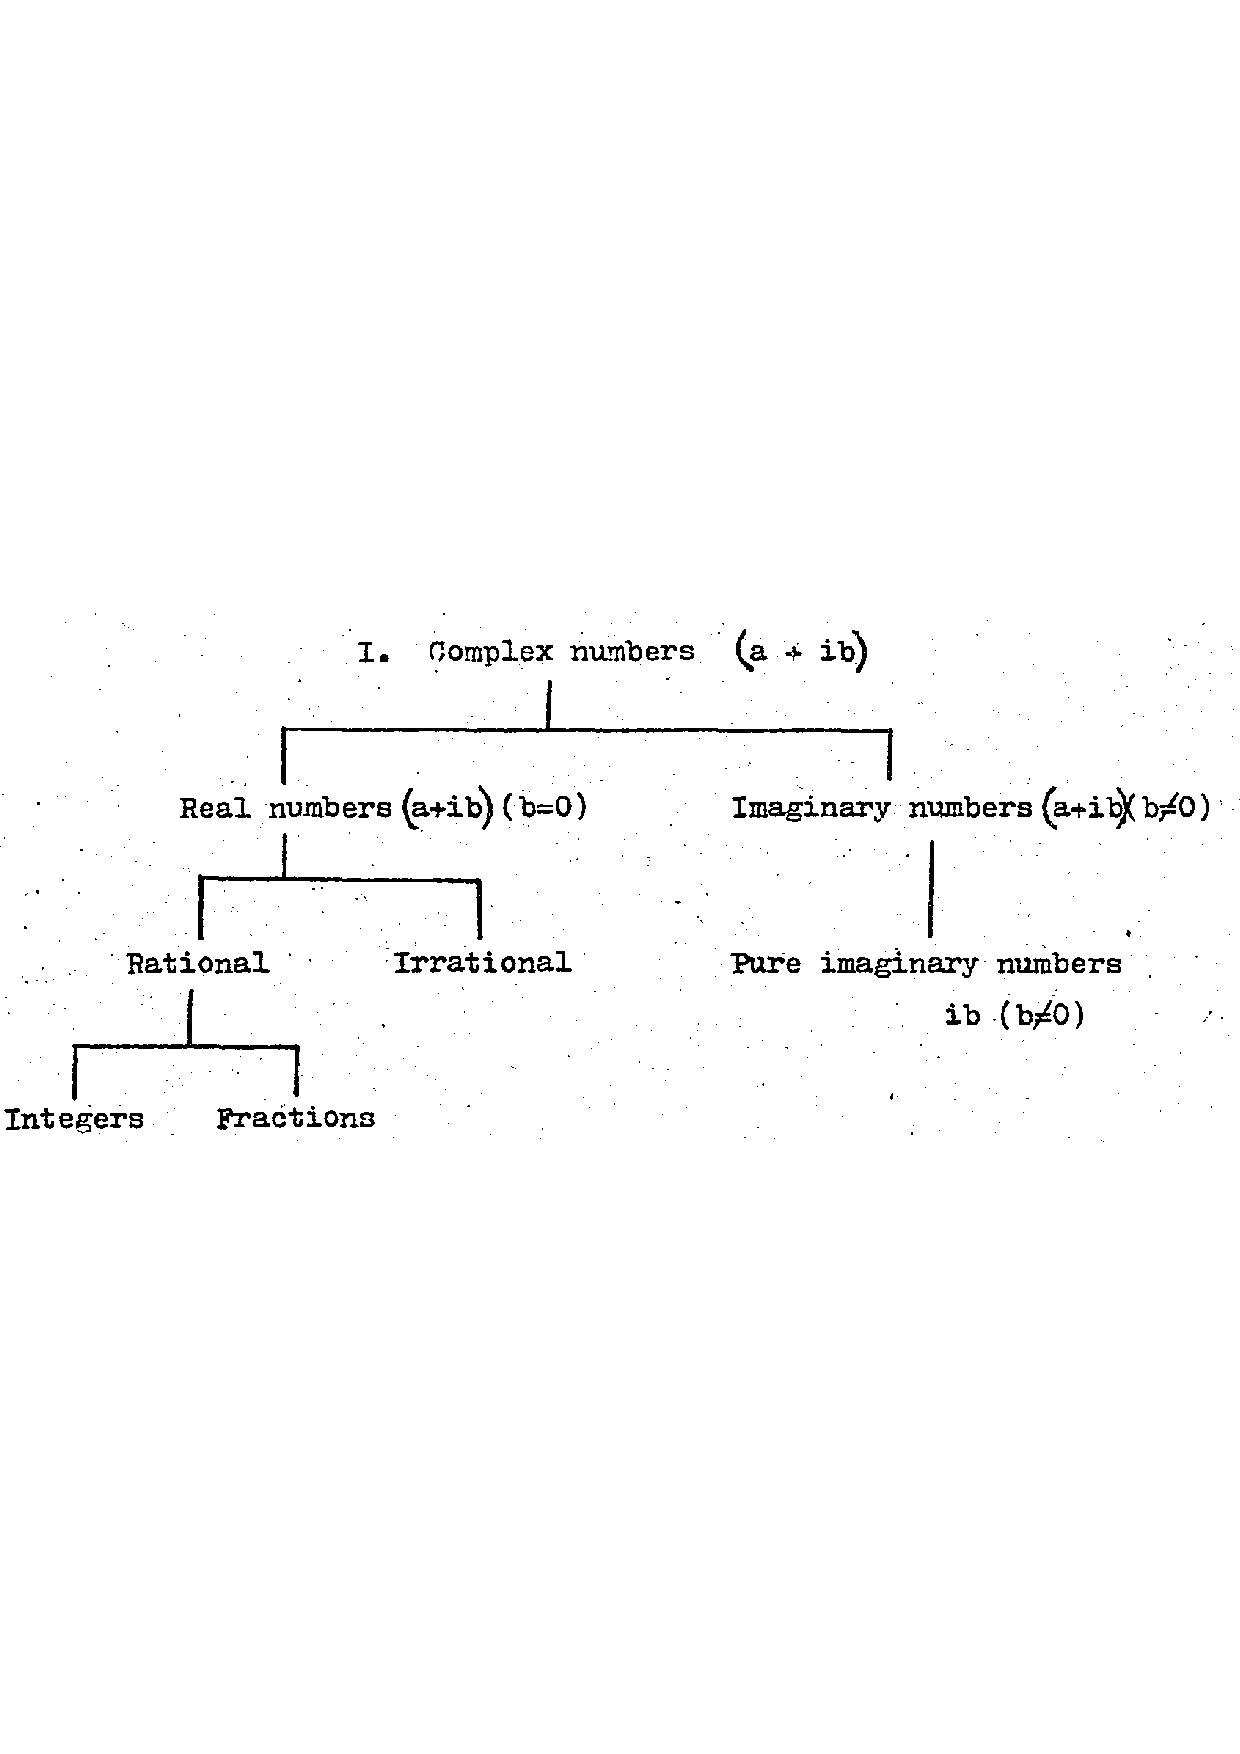
\includegraphics[width=0.9\textwidth]{images/SD-1-1p15A}
%	\caption{Classification of complex numbers}
%	\label{fig:classificationOfComplexNumbersA}
%\end{figure}

%\begin{center}
%\begin{tabular}{cc}
%\end{tabular}
%\end{center}

%\begin{exmp}
%\begin{hSolution}
%\end{hSolution}
%\end{exmp}

%\begin{hEnumerateAlpha}
%\end{hEnumerateAlpha}

%\begin{hEnumerateRoman}
%\end{hEnumerateRoman}

%$
%\begin{bmatrix}
%\end{bmatrix}
%$

%\frac{aaaa}{bbb}
%\frac{a_{n}}{b_{n}}
%\left( aaaa \right)
%\Longrightarrow

%\begin{multicols}{2}
%	bb
%\columnbreak
%	aa
%\end{multicols}
